% kapitel/typische-lineare-uebertragungsglieder.tex
\section{D\"ampfungsph\"anomene und schwingungsf\"ahige lineare \"UTG}
\label{sec:ueberschwingen-eigenfrequenz}

\subsection{Worum geht es?}
In vielen technischen Systemen (Regelkreise, Filter, mechanische Strukturen, elektrische Netzwerke)
tritt nach einer pl\"otzlichen \"Anderung des Eingangssignals (z.\,B.\ Sprung) eine dynamische
Antwort auf. Dabei beobachtet man h\"aufig:

\begin{itemize}
  \item \textbf{Schwingen/Oszillationen:} Das Ausgangssignal zeigt periodische Anteile.
  \item \textbf{\"Uberschwingen (Overshoot):} Der Ausgang \"uberschreitet kurzzeitig den sp\"ateren Endwert.
  \item \textbf{Eigenfrequenzen:} Frequenzen, bei denen das System ohne \"au\ss ere Anregung (frei) schwingt
        bzw.\ besonders stark auf Anregungen reagiert.
\end{itemize}

Wichtig: Ein \emph{PT1-System} (z.\,B.\ einfacher RC-Tiefpass) besitzt nur einen Pol und zeigt
typischerweise \emph{kein} \"Uberschwingen. \"Uberschwingen ist ein Kennzeichen von Systemen
\emph{mindestens zweiter Ordnung} (z.\,B.\ RLC-Netzwerke, PT2, viele Regelkreise).

\subsection{D\"ampfungsph\"anomene am Beispiel des PT2-Glieds}
\[
  G(p)=\frac{K}{1+2DTp+T^2p^2}.
\]
Eine h\"aufige, normierte Schreibweise ist
\begin{equation}
  G(s) = \frac{\omega_0^2}{s^2 + 2\zeta\omega_0 s + \omega_0^2}.
  \label{eq:pt2}
\end{equation}
\begin{itemize}[itemsep=2pt]
  \item $D$ \dots\ D\"ampfungsma\ss\ (entspricht $\zeta$).
  \item $T$ \dots\ Zeitkonstante (in dieser Normierung entspricht $\omega_0=\frac{1}{T}$ der unged\"ampften Eigenkreisfrequenz).
\end{itemize}
\paragraph{G\"utefaktor.}
H\"aufig wird die D\"ampfung \"uber den \textbf{G\"utefaktor} beschrieben:
\[
  Q = \frac{1}{2D}=\frac{1}{2\zeta}.
\]
Gro\ss es $Q$ bedeutet geringe D\"ampfung $\Rightarrow$ ausgepr\"agtere Resonanzspitze und tendenziell mehr \"Uberschwingen; kleines $Q$ steht f\"ur starke D\"ampfung und rasches Abklingen.


% Magnitude response of PT2 for different damping ratios D
\begin{figure}[tb]
  \centering
  \begin{tikzpicture}
    \begin{axis}[
      width=0.78\textwidth, height=0.45\textwidth,
      grid=both, grid style={line width=.1pt, draw=gray!20},
      major grid style={line width=.2pt, draw=gray!35},
      xmode=log,
      xlabel={$\omega T$}, ylabel={$L(\omega)$ / dB},
      xmin=1e-2, xmax=1e2,
      ymin=-60, ymax=20,
      axis lines=left,
      legend style={font=\small, at={(0.02,0.02)}, anchor=south west},
      tick label style={font=\small},
      label style={font=\small},
    ]
      \addplot[thick] table[x=w,y=D0.2,col sep=comma] {data/pt2_mag_bode_T1_K1_multiD.csv};
      \addlegendentry{$D=0{,}2$}
      \addplot[thick, densely dashed] table[x=w,y=D0.5,col sep=comma] {data/pt2_mag_bode_T1_K1_multiD.csv};
      \addlegendentry{$D=0{,}5$}
      \addplot[thick, dashdotted] table[x=w,y=D0.8,col sep=comma] {data/pt2_mag_bode_T1_K1_multiD.csv};
      \addlegendentry{$D=0{,}8$}
      \addplot[thick, dotted] table[x=w,y=D1.2,col sep=comma] {data/pt2_mag_bode_T1_K1_multiD.csv};
      \addlegendentry{$D=1{,}2$}
      \addplot[dashed] coordinates {(1,0) (1,0)};
    \end{axis}
  \end{tikzpicture}
  \caption{Betragsfrequenzgang eines normierten PT2-Glieds ($T=1$, $K=1$). Kleine Dämpfung erzeugt eine Resonanzüberhöhung (Peak im Betrag), die im Zeitbereich typischerweise mit starkem Überschwingen korreliert.}
  \label{fig:pt2_mag_multiD}
\end{figure}


\paragraph{Kurze Herleitung der Normform.}
Ausgehend von $G(p)=\dfrac{K}{1+2DTp+T^2p^2}$ wird der Nenner durch $T^2$ normiert:
\[
  G(s)=\frac{K}{1+2DTs+T^2s^2}
  =\frac{\tfrac{K}{T^2}}{s^2+\tfrac{2D}{T}s+\tfrac{1}{T^2}}.
\]
Durch Gleichsetzen der Nennerkoeffizienten mit der Standardform $s^2+2\zeta\omega_0 s+\omega_0^2$ folgt
\[
  \omega_0=\frac{1}{T}, \qquad \zeta = D, \qquad \frac{K}{T^2}=K\omega_0^2.
\]
Setzt man $K=1$ (normierte statische Verst\"arkung), ergibt sich direkt \eqref{eq:pt2}.

\paragraph{Sprungantwort des Standard-PT2.}
F\"ur den Einheitssprung gilt $X_e(s)=1/s$. Damit
\[
  Y(s)=G(s)X_e(s)=\frac{\omega_0^2}{s\left(s^2+2D\omega_0 s+\omega_0^2\right)}.
\]
Schreibe den Zaehler als Differenz:
\begin{align*}
  \frac{\omega_0^2}{s\left(s^2+2D\omega_0 s+\omega_0^2\right)}
  &=\frac{\left(s^2+2D\omega_0 s+\omega_0^2\right)-\left(s^2+2D\omega_0 s\right)}
          {s\left(s^2+2D\omega_0 s+\omega_0^2\right)}\\
  &=\frac{1}{s}-\frac{s^2+2D\omega_0 s}{s\left(s^2+2D\omega_0 s+\omega_0^2\right)}\\
  &=\frac{1}{s}-\frac{s+2D\omega_0}{s^2+2D\omega_0 s+\omega_0^2}.
\end{align*}
Quadratische Ergaenzung im Nenner (Schritt fuer Schritt):
\begin{align*}
  s^2+2D\omega_0 s+\omega_0^2
  &=\bigl(s^2+2D\omega_0 s+D^2\omega_0^2\bigr)
    +\omega_0^2-D^2\omega_0^2\\
  &=(s+D\omega_0)^2+\bigl(1-D^2\bigr)\omega_0^2.
\end{align*}
Zaehler in zwei Teile zerlegen:
\[
  s+2D\omega_0=(s+D\omega_0)+D\omega_0.
\]
Definiere nun $\omega_d=\omega_0\sqrt{1-D^2}$, also $(1-D^2)\omega_0^2=\omega_d^2$. Damit:
\[
  Y(s)=\frac{1}{s}-\frac{s+D\omega_0}{(s+D\omega_0)^2+\omega_d^2}
       -\frac{D\omega_0}{(s+D\omega_0)^2+\omega_d^2}.
\]
Ruecktransformation mit den bekannten Paaren (Herleitungen der Ruecktransformationen sind nicht Teil dieses Skripts):
\begin{align}
  \Laplace^{-1}\!\left\{\frac{1}{s}\right\}&=1, \tag{L1}\label{eq:laplace_pair_L1}\\
  \Laplace^{-1}\!\left\{\frac{s+a}{(s+a)^2+\omega_d^2}\right\}&=\mathrm{e}^{-a t}\cos(\omega_d t), \tag{L2}\label{eq:laplace_pair_L2}\\
  \Laplace^{-1}\!\left\{\frac{\omega_d}{(s+a)^2+\omega_d^2}\right\}&=\mathrm{e}^{-a t}\sin(\omega_d t). \tag{L3}\label{eq:laplace_pair_L3}
\end{align}
Im letzten Ausdruck stehen zwei Bruchterme mit Quadratterm im Nenner.
Der Zaehler $s+D\omega_0$ passt direkt zum Cosinus-Paar in \eqref{eq:laplace_pair_L2}.
Fuer den zweiten Bruchterm braucht man das Sinus-Paar in \eqref{eq:laplace_pair_L3}, dort steht $\omega_d$ im Zaehler.
Wir nutzen dabei die Linearitaet der Ruecktransformation:
\[
  \Laplace^{-1}\!\{c\,F(s)\}=c\,\Laplace^{-1}\!\{F(s)\}.
\]
Daher wird der Bruchterm als Konstante mal Standardform geschrieben:
\[
  \frac{D\omega_0}{(s+a)^2+\omega_d^2}
  =\frac{D\omega_0}{\omega_d}\,\frac{\omega_d}{(s+a)^2+\omega_d^2}.
\]
Herleitungen zu bekannten Fourier-Transformationspaaren finden sich z.\,B.\ in
\href{https://en.wikipedia.org/wiki/Fourier_transform#Table_of_important_Fourier_transforms}{Fourier-Transformationspaaren}.
Setze $a=D\omega_0$. Mit \eqref{eq:laplace_pair_L3} folgt:
\[
  \Laplace^{-1}\!\left\{\frac{D\omega_0}{(s+a)^2+\omega_d^2}\right\}
  =\frac{D\omega_0}{\omega_d}\,\mathrm{e}^{-a t}\sin(\omega_d t).
\]
Da $\omega_d=\omega_0\sqrt{1-D^2}$ gilt, folgt
\[
  \frac{D\omega_0}{\omega_d}=\frac{D}{\sqrt{1-D^2}}.
\]
Damit ergibt sich
\begin{equation}
  x_a(t)=1-\mathrm{e}^{-D\omega_0 t}\!\left(\cos(\omega_d t)+\frac{D}{\sqrt{1-D^2}}\sin(\omega_d t)\right),
  \qquad \omega_d=\omega_0\sqrt{1-D^2}.
  \label{eq:pt2_step_response}
\end{equation}

\paragraph{Rechenweg f\"ur einen elektrischen Schwingkreis.}
% Generic RLC series circuit as PT2 low-pass (non-floating)
\refstepcounter{figure}%
\begin{center}
  \begin{circuitikz}[american voltages, scale=1]
    \draw
      (0,0) to[sV, l=$u_\mathrm{e}$] (0,3)
      (0,3) to[R, l=$R$] (2.5,3)
      to[L, l=$L$] (5,3)
      to[C, l=$C$, v^<=$u_C$] (5,0)
      (5,0) -- (0,0);
  \end{circuitikz}
\end{center}
\vspace{-0.4em}
\noindent\textbf{Abbildung \thefigure:} Reihenschwingkreis als PT2-Tiefpass ($u_C$ als Ausgang). Die Parameter $R$, $L$, $C$ werden mit $T=\sqrt{LC}$ und $D=\tfrac{R}{2}\sqrt{\tfrac{C}{L}}$ in die Normform eingesetzt.
\label{fig:pt2_schwingkreis}


Betrachte einen Reihenschwingkreis aus $R$, $L$, $C$ (Ausgangsspannung am Kondensator, Tiefpass-PT2). Mit $Z_R=R$, $Z_L=sL$, $Z_C=\tfrac{1}{sC}$ liefert die Spannungsteilung
\[
  G(s)=\frac{U_C(s)}{U_E(s)}=\frac{Z_C}{Z_R+Z_L+Z_C}
      =\frac{\tfrac{1}{sC}}{R+sL+\tfrac{1}{sC}}
      =\frac{1}{LC\,s^2 + RC\,s + 1}.
\]
Vergleiche den Nenner mit $1+2DTs+T^2s^2$:
\[
  T^2=LC,\qquad 2DT=RC \quad\Rightarrow\quad T=\sqrt{LC},\quad D=\frac{R}{2}\sqrt{\frac{C}{L}}.
\]
Damit
\[
  \omega_0=\frac{1}{T}=\frac{1}{\sqrt{LC}},\qquad Q=\frac{1}{2D}=\sqrt{\frac{L}{C}}\frac{1}{R}.
\]
Analog verf\"ahrt man bei mechanischen Schwingkreisen (Masse--Feder--D\"ampfer), indem die Koeffizienten der Bewegungsgleichung mit der PT2-Normform abgeglichen werden.

Die Polstellen von \eqref{eq:pt2} sind
\[
  s_{1,2} = -\zeta\omega_0 \pm j\,\omega_0\sqrt{1-\zeta^2}.
\]

\paragraph{Zeitpunkt des ersten Maximums.}
Ein Maximum liegt an einer Stelle mit $\dot x_a(t)=0$. Daher leiten wir die Sprungantwort
(vgl. \eqref{eq:pt2_step_response}) ab:
\[
  \dot x_a(t)=\frac{\omega_0}{\sqrt{1-D^2}}\,\mathrm{e}^{-D\omega_0 t}\,\sin(\omega_d t).
\]
Damit gilt $\dot x_a(t)=0$ f\"ur $t=k\pi/\omega_d$; der erste positive Extremwert liegt bei $k=1$.
Die Zeit bis zum ersten Peak (peak time) ist somit
\begin{equation}
  t_p = \frac{\pi}{\omega_d} = \frac{\pi}{\omega_0\sqrt{1-D^2}}.
  \label{eq:tp}
\end{equation}

\paragraph{Einschwingzeit (Faustregel).}
Die Schwingungsamplitude folgt der H\"ulle $\mathrm{e}^{-D\omega_0 t}$.
Als 2\,\%-Einschwingzeit wird h\"aufig die Faustregel verwendet:
\begin{equation}
  t_s \approx \frac{4}{D\,\omega_0}=\frac{4T}{D}.
  \label{eq:ts}
\end{equation}
(Die N\"aherung ist am besten im mittleren D\"ampfungsbereich und dient der schnellen Absch\"atzung.)

\subsubsection{\"Uberschwingen bei der Sprungantwort}
Betrachte einen Einheitssprung $x_e(t)=\sigma(t)$ am Eingang eines stabilen Systems der Form
\eqref{eq:pt2}. F\"ur $0<D<1$ zeigt die Sprungantwort typischerweise ein Maximum oberhalb des Endwerts.

Die Sprungantwort lautet \eqref{eq:pt2_step_response}.

\paragraph{Differentialgleichung des Standard-PT2.}
Aus \eqref{eq:pt2} folgt mit $G(s)=\dfrac{Y(s)}{X_e(s)}$ und damit $Y(s)=G(s)X_e(s)$:
\[
  Y(s)=\frac{\omega_0^2}{s^2+2D\omega_0 s+\omega_0^2}\,X_e(s).
\]
Multiplikation mit dem Nenner liefert
\[
  \left(s^2+2D\omega_0 s+\omega_0^2\right)Y(s)=\omega_0^2\,X_e(s).
\]
R\"ucktransformation (bei Null-Anfangsbedingungen) liefert im Zeitbereich
\[
  \ddot x_a(t)+2D\omega_0 \dot x_a(t)+\omega_0^2 x_a(t)=\omega_0^2 x_e(t).
\]
F\"ur den Einheitssprung gilt $x_e(t)=\sigma(t)$, also
\[
  \ddot x_a+2D\omega_0 \dot x_a+\omega_0^2 x_a=\omega_0^2.
\]

\paragraph{D\"ampfungsf\"alle.}
\begin{itemize}[itemsep=2pt]
  \item $D<0$ (\emph{negative D\"ampfung}): Energiezufuhr statt Verlust, Schwingungen wachsen an (instabil).
  \item $0<D<1$ (\emph{unterd\"ampft}): komplex konjugierte Pole, schwingende Sprungantwort mit \"Uberschwingen.
  \item $D=1$ (\emph{kritisch ged\"ampft}): Doppelpol, schnell ohne \"Uberschwingen (Grenzfall).
  \item $D>1$ (\emph{\"uberd\"ampft}): zwei reelle Pole, monotone Sprungantwort ohne \"Uberschwingen.
\end{itemize}

% Step response of PT2 for different damping ratios D
\begin{figure}[tb]
  \centering
  \begin{tikzpicture}
    \begin{axis}[
      width=0.78\textwidth, height=0.45\textwidth,
      grid=both, grid style={line width=.1pt, draw=gray!20},
      major grid style={line width=.2pt, draw=gray!35},
      xlabel={$t/T$}, ylabel={$x_a(t)/K$},
      xmin=0, xmax=20,
      ymin=-0.05, ymax=1.8,
      axis lines=left,
      legend style={font=\small, at={(0.98,0.02)}, anchor=south east},
      tick label style={font=\small},
      label style={font=\small},
    ]
      \addplot[thick] table[x=t,y=D0.2,col sep=comma] {data/pt2_step_T1_K1_multiD.csv};
      \addlegendentry{$D=0{,}2$}
      \addplot[thick, densely dashed] table[x=t,y=D0.5,col sep=comma] {data/pt2_step_T1_K1_multiD.csv};
      \addlegendentry{$D=0{,}5$}
      \addplot[thick, dashdotted] table[x=t,y=D0.8,col sep=comma] {data/pt2_step_T1_K1_multiD.csv};
      \addlegendentry{$D=0{,}8$}
      \addplot[thick, dotted] table[x=t,y=D1.0,col sep=comma] {data/pt2_step_T1_K1_multiD.csv};
      \addlegendentry{$D=1{,}0$}
      \addplot[thick] table[x=t,y=D1.2,col sep=comma] {data/pt2_step_T1_K1_multiD.csv};
      \addlegendentry{$D=1{,}2$}
      \addplot[dashed] coordinates {(0,1) (20,1)};
    \end{axis}
  \end{tikzpicture}
  \caption{Sprungantwort eines normierten PT2-Glieds ($T=1$, $K=1$) f\"ur unterschiedliche D\"ampfungsma\ss e $D$. Unterd\"ampfung ($D<1$) f\"uhrt zu \"Uberschwingen und Schwingungen; bei $D\ge1$ verschwindet das \"Uberschwingen.}
  \label{fig:pt2_step_multiD}
\end{figure}

\FloatBarrier

\textbf{\"Uberschwingma\ss} (relative peak overshoot) $M_p$:
\[
  M_p = \frac{x_{a,\text{max}}-\lim_{t\to\infty}x_a(t)}{\lim_{t\to\infty}x_a(t)}.
\]
Oft wird es in Prozent angegeben: $M_p[\%] = 100\cdot M_p$.

F\"ur das Standard-PT2 gilt (bei Einheitssprung, $0<D<1$):
\begin{equation}
  M_p=\exp\!\left(-\frac{D\pi}{\sqrt{1-D^2}}\right).
  \label{eq:overshoot}
\end{equation}
Herleitung (kurz): Mit \eqref{eq:pt2_step_response} und $t_p=\pi/\omega_d$ (siehe \eqref{eq:tp}) folgt
\[
  x_a(t_p)=1-\mathrm{e}^{-D\omega_0 t_p}\cos(\pi)=1+\mathrm{e}^{-D\omega_0 t_p},
\]
und somit
\[
  M_p=\frac{x_a(t_p)-1}{1}=\mathrm{e}^{-D\omega_0 t_p}
  =\exp\!\left(-D\omega_0\cdot\frac{\pi}{\omega_0\sqrt{1-D^2}}\right)
  =\exp\!\left(-\frac{D\pi}{\sqrt{1-D^2}}\right).
\]
Umgekehrt:
\[
  \ln(M_p)=-\frac{D\pi}{\sqrt{1-D^2}}
  \ \Rightarrow\ 
  \ln^2(M_p)=\frac{D^2\pi^2}{1-D^2}
  \ \Rightarrow\ 
  D^2=\frac{\ln^2(M_p)}{\pi^2+\ln^2(M_p)}.
\]
\[
  D=\frac{-\ln(M_p)}{\sqrt{\pi^2+\ln^2(M_p)}}.
\]

\paragraph{Logarithmisches Daempfungsdekrement.}
F\"ur eine unterd\"ampfte PT2-Sprungantwort bezeichnen $x_k$ und $x_{k+1}$ zwei aufeinanderfolgende
Maxima, $x_\infty$ den Endwert. Dann ist das logarithmische Daempfungsdekrement
\[
  \Lambda=\ln\!\left(\frac{x_k-x_\infty}{x_{k+1}-x_\infty}\right)
  =\frac{2\pi D}{\sqrt{1-D^2}}.
\]
Herleitung (kurz): F\"ur den normierten PT2 und den Einheitssprung $x_e(t)=\sigma(t)$ gilt im Zeitbereich
\[
  \ddot x_a + 2D\omega_0 \dot x_a + \omega_0^2 x_a = \omega_0^2.
\]
Homogene Gleichung: Ansatz $x_h=\mathrm{e}^{s t}$ liefert die charakteristische Gleichung
\[
  s^2+2D\omega_0 s+\omega_0^2=0,
\]
deren L\"osungen $s_{1,2}=-D\omega_0\pm \jj\,\omega_d$ mit $\omega_d=\omega_0\sqrt{1-D^2}$ sind.
Zu jedem Eigenwert $s_i$ geh\"ort ein Summand $\mathrm{e}^{s_i t}$, daher
\[
  x_h(t)=C_1\,\mathrm{e}^{s_1 t}+C_2\,\mathrm{e}^{s_2 t}.
\]
Einsetzen von $s_{1,2}$ ergibt
\[
  x_h(t)=C_1\,\mathrm{e}^{(-D\omega_0+\jj\omega_d)t}+C_2\,\mathrm{e}^{(-D\omega_0-\jj\omega_d)t}.
\]
Aus $\mathrm{e}^{(a+b)t}=\mathrm{e}^{a t}\mathrm{e}^{b t}$ folgt durch Ausklammern von
$\mathrm{e}^{-D\omega_0 t}$:
\[
  x_h(t)=\mathrm{e}^{-D\omega_0 t}\bigl(C_1\,\mathrm{e}^{\jj\omega_d t}+C_2\,\mathrm{e}^{-\jj\omega_d t}\bigr).
\]
Mit der Euler-Formel fasst man die komplexen Exponentialanteile zu Cosinus und Sinus zusammen:
\[
  x_h(t)=\mathrm{e}^{-D\omega_0 t}\bigl(A\cos(\omega_d t)+B\sin(\omega_d t)\bigr).
\]
Dabei gilt explizit
\[
  \mathrm{e}^{\jj\omega_d t}=\cos(\omega_d t)+\jj\sin(\omega_d t),\qquad
  \mathrm{e}^{-\jj\omega_d t}=\cos(\omega_d t)-\jj\sin(\omega_d t),
\]
so dass sich die reelle Linearkombination in Cosinus- und Sinusanteile zerlegt.
Die Gesamtl\"osung ist die Summe aus homogener und partikul\"arer L\"osung:
\[
  x_a(t)=x_h(t)+x_p(t).
\]
Die partikul\"are L\"osung ist der station\"are Anteil und gilt f\"ur alle Zeiten als
$x_a(t)=x_p(t)+x_h(t)$. Bei stabilem System verschwindet der transiente Anteil
$x_h(t)$ f\"ur $t\to\infty$, sodass dann $x_a(t)\to x_p(t)$.
Rechte Seite ist konstant $\Rightarrow$ der station\"are Anteil ist konstant; daraus folgt
$x_p(t)=x_\infty=1$.
Damit gilt $x_a(t)-x_\infty=x_h(t)$. Die Linearkombination l\"asst sich zu einer Sinusform
zusammenfassen, denn
\[
  A\cos(\omega_d t)+B\sin(\omega_d t)=R\sin(\omega_d t+\varphi).
\]
Beweis: Setze $R=\sqrt{A^2+B^2}$ und w\"ahle $\varphi$ mit
\[
  R\sin\varphi=A,\qquad R\cos\varphi=B \quad (\tan\varphi=A/B).
\]
Dann gilt
\[
  R\sin(\omega_d t+\varphi)
  =R\bigl(\sin(\omega_d t)\cos\varphi+\cos(\omega_d t)\sin\varphi\bigr)
  =R\sin(\omega_d t)\cos\varphi+R\cos(\omega_d t)\sin\varphi
  =B\sin(\omega_d t)+A\cos(\omega_d t).
\]
Daher gilt fuer die Abweichung
\[
  x_a(t)-x_\infty=\mathrm{e}^{-D\omega_0 t}\bigl(A\cos(\omega_d t)+B\sin(\omega_d t)\bigr),
\]
und damit kann man schreiben
\[
  x_a(t)-x_\infty = R\,\mathrm{e}^{-D\omega_0 t}\sin(\omega_d t+\varphi).
\]
Sei $t_k$ der Zeitpunkt des $k$-ten Maximums der Sprungantwort, dann ist
$x_k=x_a(t_k)$ und $x_\infty=\lim_{t\to\infty}x_a(t)$ der Endwert. Aus
\[
  x_a(t)-x_\infty=R\,\mathrm{e}^{-D\omega_0 t}\sin(\omega_d t+\varphi)
\]
folgt an einem Maximum $\sin(\omega_d t_k+\varphi)=1$ und damit
\[
  x_k-x_\infty=R\,\mathrm{e}^{-D\omega_0 t_k}.
\]
Der Sinus hat die Periode $T_d=\frac{2\pi}{\omega_d}$, daher liegen aufeinanderfolgende Maxima
um genau eine Periode auseinander: $t_{k+1}-t_k=T_d$. Damit
\[
  \frac{x_k-x_\infty}{x_{k+1}-x_\infty}
  =\frac{R\,\mathrm{e}^{-D\omega_0 t_k}}{R\,\mathrm{e}^{-D\omega_0 t_{k+1}}}
  =\exp\!\bigl(D\omega_0(t_{k+1}-t_k)\bigr)
  =\exp\!\left(D\omega_0\frac{2\pi}{\omega_d}\right),
\]
und mit $\omega_d=\omega_0\sqrt{1-D^2}$ folgt
\[
  \Lambda=\ln\!\left(\frac{x_k-x_\infty}{x_{k+1}-x_\infty}\right)
  =\frac{2\pi D}{\sqrt{1-D^2}}.
\]
Zusammenhang zum \"Uberschwingma\ss: F\"ur den normierten Endwert $x_\infty=1$ gilt
\[
  M_p=\exp\!\left(-\frac{D\pi}{\sqrt{1-D^2}}\right)=\exp\!\left(-\frac{\Lambda}{2}\right),
  \qquad
  \Lambda=2\ln\!\left(\frac{1}{M_p}\right).
\]
Warum logarithmisch? Die H\"ullkurve der Schwingungsamplitude f\"allt exponentiell, d.\,h.\ die
Verh\"altnisse aufeinanderfolgender Maxima sind konstant. Der Logarithmus macht diese
multiplikative Abnahme additiv und unabh\"angig von der Anfangsamplitude. Vorteil: $D$ l\"asst
sich direkt aus zwei (oder mehreren gemittelten) Peaks robust bestimmen.

% Logarithmisches Daempfungsdekrement an einer unterdaempften PT2-Sprungantwort
\begin{figure}[!ht]
  \centering
  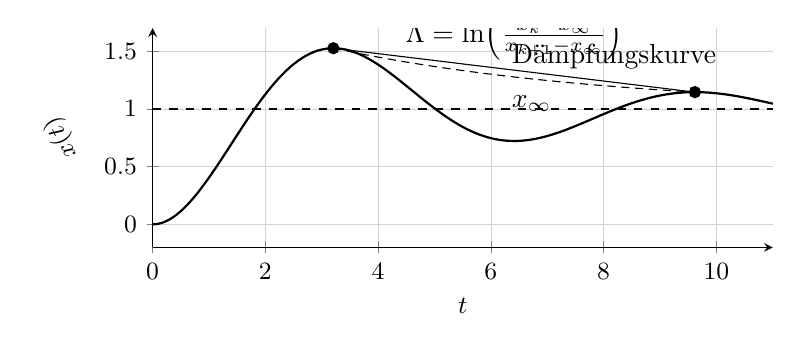
\begin{tikzpicture}
    \pgfmathsetmacro{\damp}{0.2}
    \pgfmathsetmacro{\omegad}{sqrt(1-\damp*\damp)}
    \pgfmathsetmacro{\tpeakone}{pi/\omegad}
    \pgfmathsetmacro{\tpeaktwo}{\tpeakone + 2*pi/\omegad}
    \pgfmathsetmacro{\mpeak}{exp(-\damp*pi/\omegad)}
    \pgfmathsetmacro{\xone}{1 + \mpeak}
    \pgfmathsetmacro{\xtwo}{1 + \mpeak*exp(-2*pi*\damp/\omegad)}
    \begin{axis}[
      width=0.78\textwidth, height=0.36\textwidth,
      grid=both, grid style={line width=.1pt, draw=gray!20},
      major grid style={line width=.2pt, draw=gray!35},
      xlabel={$t$}, ylabel={$x(t)$},
      xmin=0, xmax=11,
      ymin=-0.2, ymax=1.7,
      axis lines=left,
      tick label style={font=\small},
      label style={font=\small},
      trig format=rad
    ]
      \addplot[thick, domain=0:11, samples=400]
        {1 - exp(-\damp*x)*(cos(\omegad*x) + (\damp/\omegad)*sin(\omegad*x))};
      \addplot[dashed] coordinates {(0,1) (11,1)};
      % Daempfungskurve zwischen zwei Maxima (Envelope der Peak-Abstaende)
      \addplot[densely dashed, domain=\tpeakone:\tpeaktwo]
        {1 + \mpeak*exp(-\damp*(x-\tpeakone))};
      \addplot[only marks, mark=*] coordinates {(\tpeakone,\xone) (\tpeaktwo,\xtwo)};
      \draw[->] (axis cs:\tpeakone,\xone) -- (axis cs:\tpeaktwo,\xtwo)
        node[midway, above] {$\Lambda=\ln\!\left(\frac{x_k-x_\infty}{x_{k+1}-x_\infty}\right)$};
      \node[anchor=west] at (axis cs:6.2,1.05) {$x_\infty$};
      \node[anchor=west] at (axis cs:6.2,1.45) {D\"ampfungskurve};
    \end{axis}
  \end{tikzpicture}
  \caption{Unterd\"ampfte PT2-Sprungantwort: Das logarithmische Daempfungsdekrement $\Lambda$ ergibt sich aus zwei aufeinanderfolgenden Maxima der Abweichung von $x_\infty$.}
  \label{fig:log_decrement}
\end{figure}


\paragraph{Beispiel (\"Uberschwingen).}
F\"ur $D=0{,}5$ ergibt sich
$M_p=\exp\!\left(-\frac{0{,}5\pi}{\sqrt{1-0{,}25}}\right)\approx 0{,}16$,
also etwa $16\,\%$ \"Uberschwingen.

% Overshoot vs damping ratio
\begin{figure}[tb]
  \centering
  \begin{tikzpicture}
    \begin{axis}[
      width=0.70\textwidth, height=0.42\textwidth,
      grid=both, grid style={line width=.1pt, draw=gray!20},
      major grid style={line width=.2pt, draw=gray!35},
      xlabel={Dämpfungsmaß $D$}, ylabel={$M_p$ / \%},
      xmin=0, xmax=1,
      ymin=0, ymax=110,
      axis lines=left,
      tick label style={font=\small},
      label style={font=\small},
    ]
      \addplot[thick] table[x=D,y=Mp_percent,col sep=comma] {data/pt2_overshoot_vs_damping.csv};
      \addplot[dashed] coordinates {(0.5,0) (0.5,110)};
      \node[anchor=west, font=\small] at (axis cs:0.51,70) {$D=0{,}5 \Rightarrow M_p\approx16\%$};
    \end{axis}
  \end{tikzpicture}
  \caption{Relatives Überschwingen $M_p=\exp\!\left(-\frac{D\pi}{\sqrt{1-D^2}}\right)$ (unterdämpfter Fall $0<D<1$). Mit wachsender Dämpfung sinkt das Überschwingen stark.}
  \label{fig:overshoot_vs_damping}
\end{figure}


\subsubsection{Eigenfrequenz vs.\ Resonanzfrequenz}
Die \textbf{Eigenfrequenz} beschreibt das freie Schwingverhalten (durch die Pole bestimmt).
Die \textbf{Resonanzfrequenz} beschreibt dagegen die Frequenz, bei der die \emph{erzwungene} Antwort
(z.\,B.\ Sinusanregung) maximal wird.

F\"ur das System \eqref{eq:pt2} zeigt die Betragsfrequenzgangkurve $|G(j\omega)|$ nur dann eine ausgepr\"agte
Resonanzspitze, wenn die D\"ampfung klein genug ist (typisch $D < 1/\sqrt{2}$).
Dann gilt n\"aherungsweise:
\begin{equation}
  \omega_r = \omega_0\sqrt{1-2D^2}
  \qquad (D < 1/\sqrt{2}).
  \label{eq:omega_r}
\end{equation}
Man sieht: $\omega_r$ liegt dann \emph{unter} $\omega_0$.
Kleine D\"ampfung erzeugt eine Resonanzspitze im Betragsfrequenzgang in der N\"ahe von
$\omega\approx\omega_0$. Diese Resonanz\"uberh\"ohung korreliert h\"aufig mit starkem
\"Uberschwingen im Zeitbereich.
